\section{Bestimmung der Kernladungszahl von Aluminium}
%kurz das ziel dieses versuchsteiles ansprechen, damit keine zwei �berschriften direkt �bereinander stehen!
%bei schwierigeren versuchen kann auch der theoretische hintergrund erl�utert werden. (mit formeln, herleitungen und erkl�rungen)
Es soll die Kernladungszahl von Aluminium bestimmt werden. Die Winkelverteilung der Z�hlraten soll mit denen der Goldfolie verglichen werden.


Die Aluminiumfolie mit einer Dicke von 7$\mu$m und der 1mm Spalt werden eingesetzt. Die Rutherfordkammer wird auf einen Druck von 25 mbar evakuiert. Dann werden die Z�hlraten in 5$^\circ$ Schritten �ber einen Zeitraum von 3min aufgenommen. Die Kernladungszahl wird mit  Gl. \ref{eqn:alu_kern} bestimmt. Dabei werden f�r die festen Parameter die Werte in Tabelle \ref{tab:alu_paras} verwendet.

\begin{align}
\label{eqn:alu_kern}
\frac{\text{\.{N$_{Al}$}}}{\text{\.{N$_{Au}$}}} = \frac{Z_{Al}^2 \cdot d_{Al}}{Z_{Au}^2 \cdot d_{Au}}
\end{align}

\begin{table}[H]
\centering
\caption{Werte der festen Parameter f�r die Bestimmung der Kernladungszahl von Aluminium nach Gleichung \ref{eqn:n_dot}}
\label{tab:alu_paras}
\begin{tabular}{|c|c|}
\hline Parameter & Wert \\ 
\hline $Z^2_{Au}$ & 79 \\ 
\hline $d_{Au}$ & 2 [$\mu$m] \\ 
\hline $d_{Al}$ & 7 [$\mu$m] \\ 
\hline 
\end{tabular} 
\end{table}

Dabei ist die Anzahl der Gemessenen Ereignisse \.{N} gegeben durch Gl. \ref{eqn:n_dot}.

\begin{align}
\label{eqn:n_dot}
\text{\.{N$_i$}} \propto \frac{A_i}{sin^4 \left( \frac{\Theta}{2} \right)}
\end{align}

Setzt man Gl. \ref{eqn:n_dot} in Gl. \ref{eqn:alu_kern} ein und formt nach Z$_{Al}$ um so ergibt sich die Kernladungszahl von Aluminium nach Gl. \ref{eqn:alu}

\begin{align}
\label{eqn:alu}
Z_{Al} = Z_{Au} \sqrt{\frac{A_{Al} \cdot d_{Au}}{A_{Au} \cdot d_{Al}}}
\end{align}

Der Fehler ergibt sich dabei mit nach Gl. \ref{eqn:delta_alu}.

\begin{align}
\label{eqn:delta_alu}
\Delta Z_{Al} = \sqrt{ \left( \frac{Z_{Au}^2 \cdot A_{Al} \cdot d_{Au}}{4 \cdot A_{Au} \cdot d_{Al}} \right) \left[ \left( \frac{\Delta A_{Al} \cdot d_{Au}}{A_{Al}} \right)^2 + \left( \frac{\Delta A_{Au} \cdot d_{Al}}{A_{Au}} \right)^2 \right]}
\end{align}

A$_{AL,Au}$ wird dabei aus den Fits entnommen. Die Messwerte der Rutherfordstreuung an Aluminium und der Fit sind in Abb. \ref{fig:rutherford_alu} zu sehen. F�r den Fit ergeben sich die Werte in Tabelle \ref{fig:rutherford_alu}.

\begin{figure}[H]
	\centering
  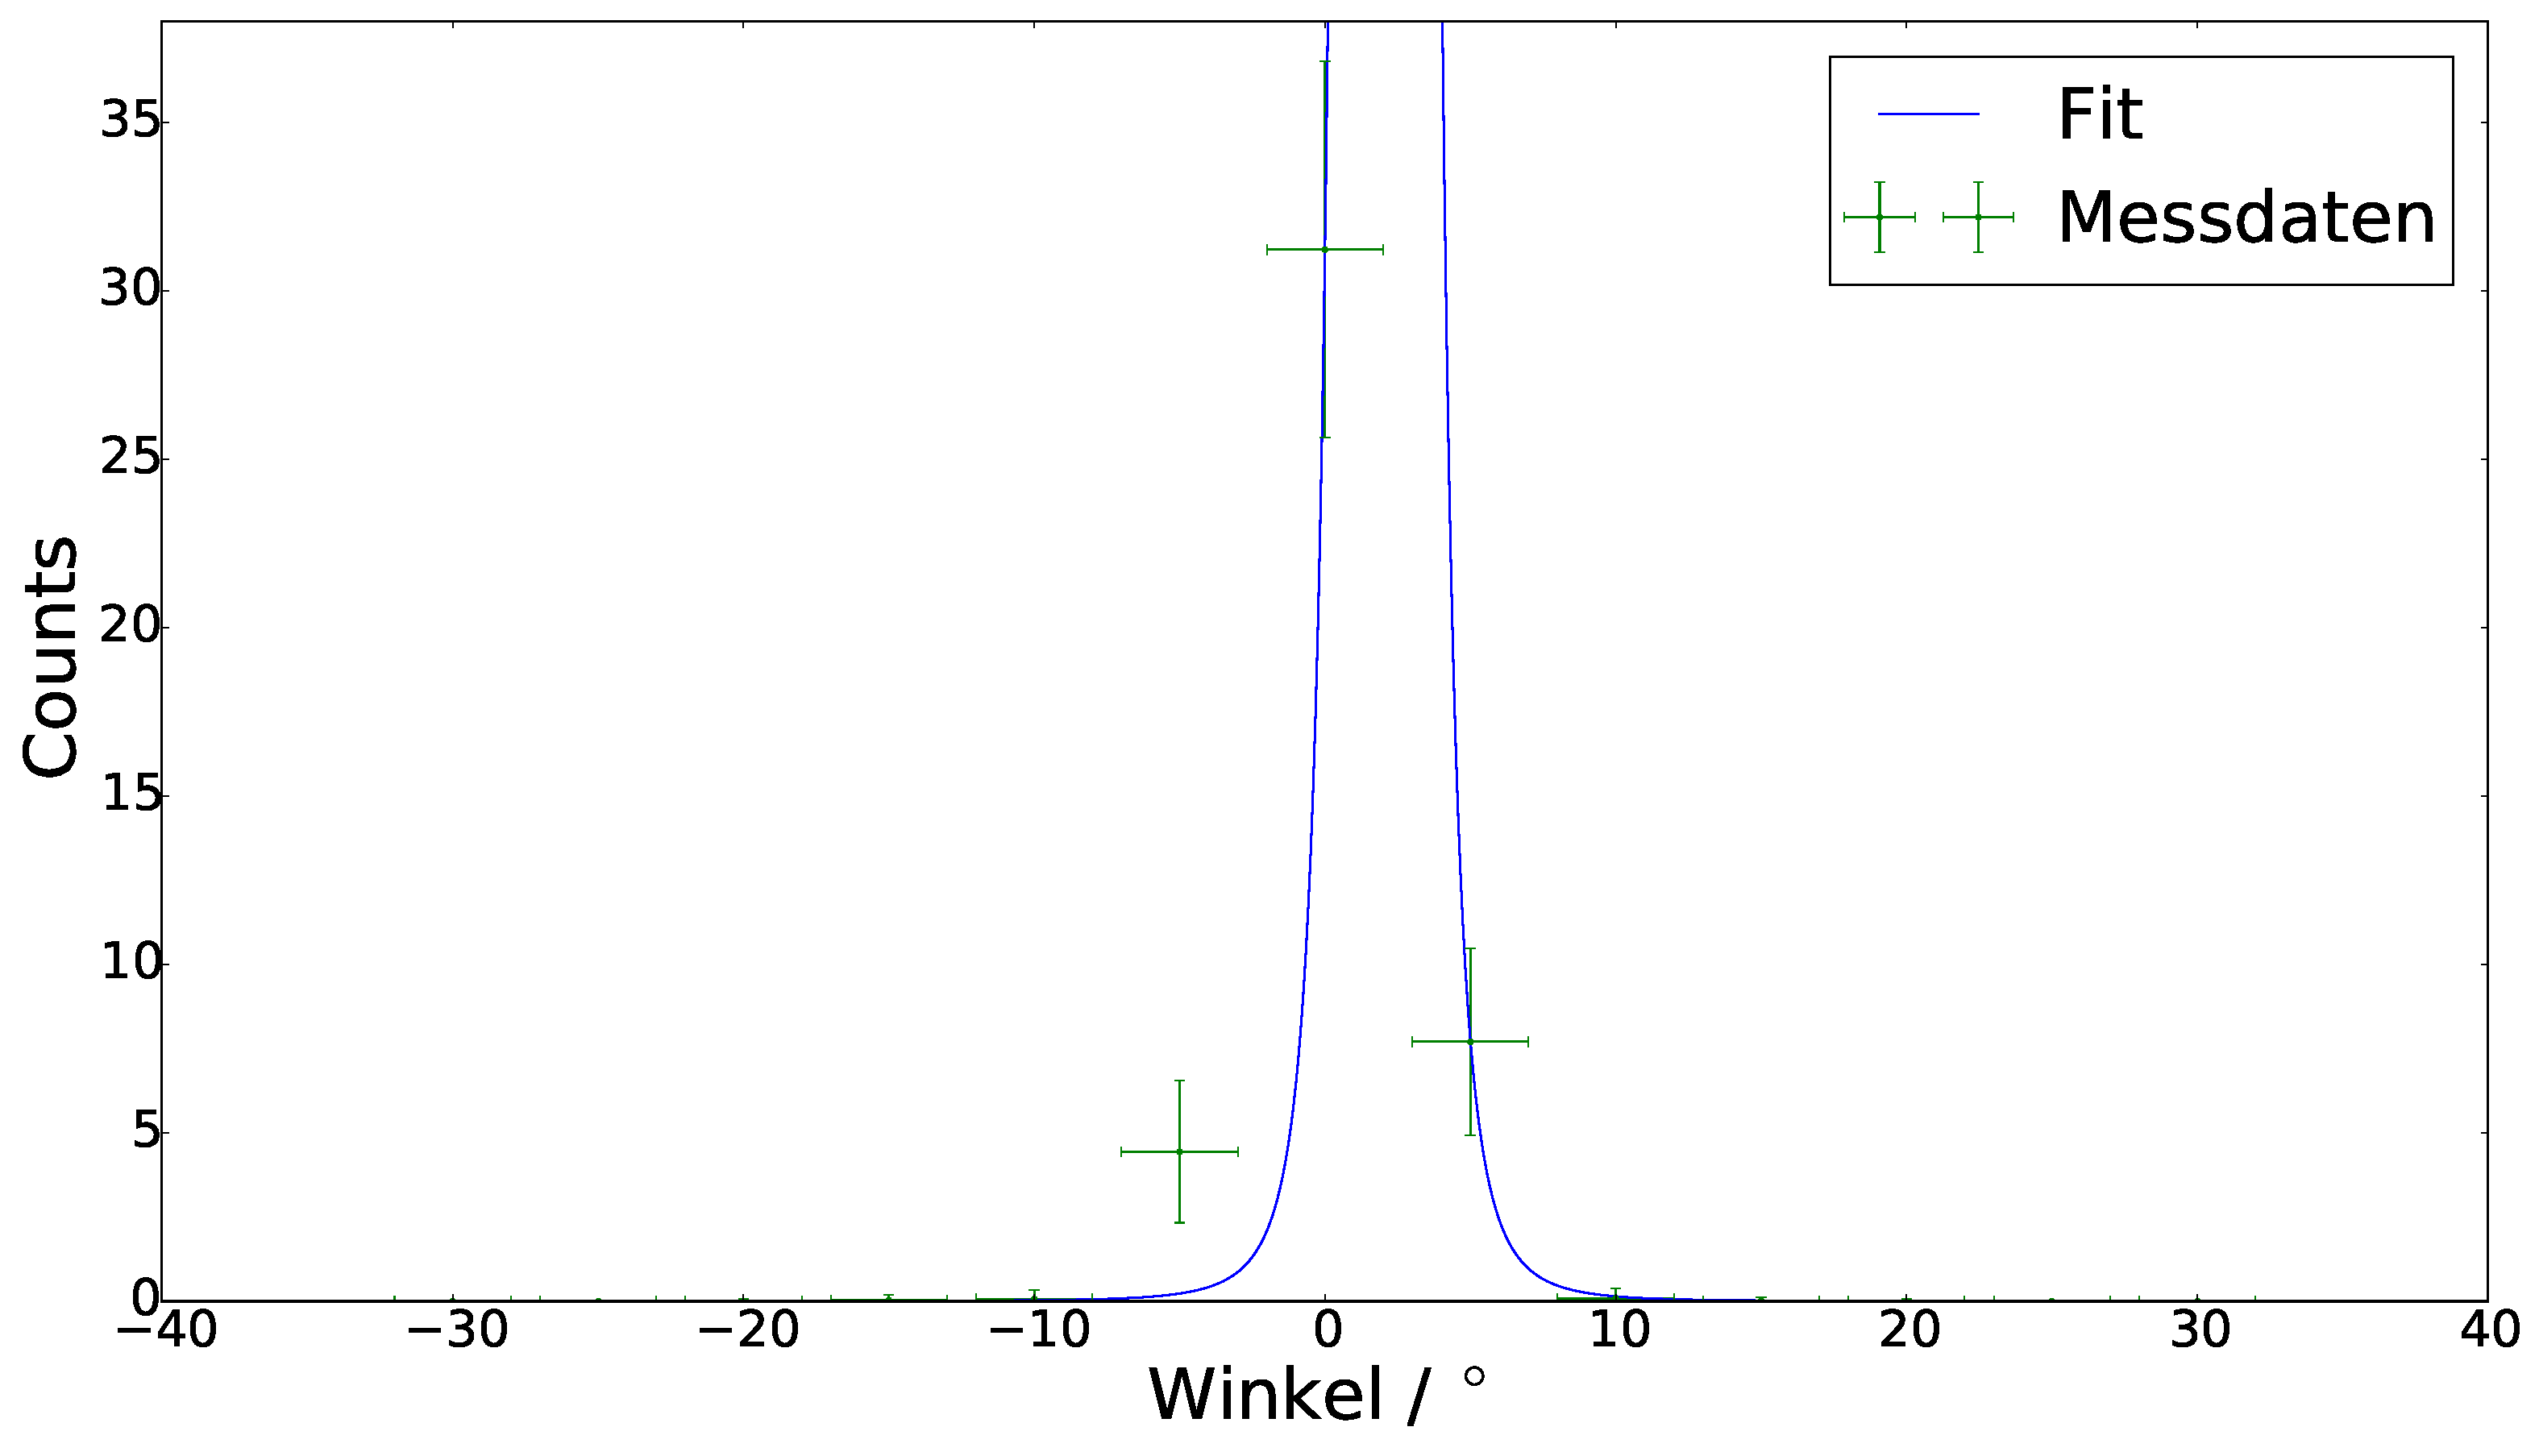
\includegraphics[scale=0.33]{rutherford_messung_alu.pdf}
	\caption{Es sind die Messdaten aus der Streuung von $\alpha$-Strahlung an Gold zu sehen. Die Messdaten wurden mit  Gl. \ref{eqn:ruth} gefittet, dabei ergab sich ein $\chi_{red}^2$ von 1,61. Optisch passt der Fit sehr gut zu den Daten, abgesehn von dem Messwert bei -5$^\circ$}
	\label{fig:rutherford_alu}
\end{figure}

\begin{table}
\centering
\caption{Fitparamter f�r das Aluminiumatom nach Gl. \ref{eqn:ruth}}
\label{tab:fit_alu_ruth}
\begin{tabular}{|c|c|}
\hline Paramter & Wert \\ 
\hline A & 0,000033 $\pm$ 0,000003 \\ 
\hline B & 2,07 $\pm$ 0,05 \\ 
\hline $\chi_{red}^2$ & 1,61 \\ 
\hline 
\end{tabular} 
\end{table}

Setzt man die Fitparameter aus Tabelle \ref{fig:rutherford_gold} und Tabelle \ref{tab:fit_alu_ruth} in Gl. \ref{eqn:alu} ein so ergibt sich ein Kernladung von 12,6 $\pm$ 0,3. Erwartet wurde ein Wert von 13, der bestimmte Werte weicht um 0.97\% von dem Erwartetem ab. Das Ergebnis ist im Rahmen der Messung als gut einzuordnen.

%Vergleich der beiden Werte